% Options for packages loaded elsewhere
\PassOptionsToPackage{unicode}{hyperref}
\PassOptionsToPackage{hyphens}{url}
\PassOptionsToPackage{dvipsnames,svgnames,x11names}{xcolor}
%
\documentclass[
  12pt,
]{article}

\usepackage{amsmath,amssymb}
\usepackage[]{crimson}
\usepackage{setspace}
\usepackage{iftex}
\ifPDFTeX
  \usepackage[T1]{fontenc}
  \usepackage[utf8]{inputenc}
  \usepackage{textcomp} % provide euro and other symbols
\else % if luatex or xetex
  \usepackage{unicode-math}
  \defaultfontfeatures{Scale=MatchLowercase}
  \defaultfontfeatures[\rmfamily]{Ligatures=TeX,Scale=1}
\fi
% Use upquote if available, for straight quotes in verbatim environments
\IfFileExists{upquote.sty}{\usepackage{upquote}}{}
\IfFileExists{microtype.sty}{% use microtype if available
  \usepackage[]{microtype}
  \UseMicrotypeSet[protrusion]{basicmath} % disable protrusion for tt fonts
}{}
\usepackage{xcolor}
\usepackage[margin = 1in]{geometry}
\setlength{\emergencystretch}{3em} % prevent overfull lines
\setcounter{secnumdepth}{5}
% Make \paragraph and \subparagraph free-standing
\ifx\paragraph\undefined\else
  \let\oldparagraph\paragraph
  \renewcommand{\paragraph}[1]{\oldparagraph{#1}\mbox{}}
\fi
\ifx\subparagraph\undefined\else
  \let\oldsubparagraph\subparagraph
  \renewcommand{\subparagraph}[1]{\oldsubparagraph{#1}\mbox{}}
\fi


\providecommand{\tightlist}{%
  \setlength{\itemsep}{0pt}\setlength{\parskip}{0pt}}\usepackage{longtable,booktabs,array}
\usepackage{calc} % for calculating minipage widths
% Correct order of tables after \paragraph or \subparagraph
\usepackage{etoolbox}
\makeatletter
\patchcmd\longtable{\par}{\if@noskipsec\mbox{}\fi\par}{}{}
\makeatother
% Allow footnotes in longtable head/foot
\IfFileExists{footnotehyper.sty}{\usepackage{footnotehyper}}{\usepackage{footnote}}
\makesavenoteenv{longtable}
\usepackage{graphicx}
\makeatletter
\def\maxwidth{\ifdim\Gin@nat@width>\linewidth\linewidth\else\Gin@nat@width\fi}
\def\maxheight{\ifdim\Gin@nat@height>\textheight\textheight\else\Gin@nat@height\fi}
\makeatother
% Scale images if necessary, so that they will not overflow the page
% margins by default, and it is still possible to overwrite the defaults
% using explicit options in \includegraphics[width, height, ...]{}
\setkeys{Gin}{width=\maxwidth,height=\maxheight,keepaspectratio}
% Set default figure placement to htbp
\makeatletter
\def\fps@figure{htbp}
\makeatother

\usepackage{booktabs}
\usepackage{longtable}
\usepackage{array}
\usepackage{multirow}
\usepackage{wrapfig}
\usepackage{float}
\usepackage{colortbl}
\usepackage{pdflscape}
\usepackage{tabu}
\usepackage{threeparttable}
\usepackage{threeparttablex}
\usepackage[normalem]{ulem}
\usepackage{makecell}
\usepackage{xcolor}
\usepackage[scale = 0.8]{sourcecodepro}
\usepackage{etoolbox}
\makeatletter
\makeatother
\makeatletter
\makeatother
\makeatletter
\@ifpackageloaded{caption}{}{\usepackage{caption}}
\AtBeginDocument{%
\ifdefined\contentsname
  \renewcommand*\contentsname{Table of contents}
\else
  \newcommand\contentsname{Table of contents}
\fi
\ifdefined\listfigurename
  \renewcommand*\listfigurename{List of Figures}
\else
  \newcommand\listfigurename{List of Figures}
\fi
\ifdefined\listtablename
  \renewcommand*\listtablename{List of Tables}
\else
  \newcommand\listtablename{List of Tables}
\fi
\ifdefined\figurename
  \renewcommand*\figurename{Figure}
\else
  \newcommand\figurename{Figure}
\fi
\ifdefined\tablename
  \renewcommand*\tablename{Table}
\else
  \newcommand\tablename{Table}
\fi
}
\@ifpackageloaded{float}{}{\usepackage{float}}
\floatstyle{ruled}
\@ifundefined{c@chapter}{\newfloat{codelisting}{h}{lop}}{\newfloat{codelisting}{h}{lop}[chapter]}
\floatname{codelisting}{Listing}
\newcommand*\listoflistings{\listof{codelisting}{List of Listings}}
\makeatother
\makeatletter
\@ifpackageloaded{caption}{}{\usepackage{caption}}
\@ifpackageloaded{subcaption}{}{\usepackage{subcaption}}
\makeatother
\makeatletter
\@ifpackageloaded{tcolorbox}{}{\usepackage[many]{tcolorbox}}
\makeatother
\makeatletter
\@ifundefined{shadecolor}{\definecolor{shadecolor}{rgb}{.97, .97, .97}}
\makeatother
\makeatletter
\makeatother
\ifLuaTeX
  \usepackage{selnolig}  % disable illegal ligatures
\fi
\IfFileExists{bookmark.sty}{\usepackage{bookmark}}{\usepackage{hyperref}}
\IfFileExists{xurl.sty}{\usepackage{xurl}}{} % add URL line breaks if available
\urlstyle{same} % disable monospaced font for URLs
\hypersetup{
  pdftitle={See the Other Side: Local Party Images and Affective Polarization},
  pdfauthor={Chaoyue Wang},
  colorlinks=true,
  linkcolor={RoyalBlue4},
  filecolor={Maroon},
  citecolor={RoyalBlue4},
  urlcolor={Cyan4},
  pdfcreator={LaTeX via pandoc}}

\title{See the Other Side: Local Party Images and Affective
Polarization}
\author{Chaoyue Wang\footnote{Chaoyue R. Wang
  (\texttt{chyrwang@gmail.com}, \texttt{86-177-2387-5369}) is a senior
  student of Philosophy, Politics and Economics at Yuanpei College of
  Peking University, Beijing, China 100871.}}
\date{October 8, 2022}

\begin{document}
\maketitle

%----------------------------------------------
%   Abstract
%----------------------------------------------

\thispagestyle{empty}

\begin{abstract}  \onehalfspacing
\begin{normalsize}  \noindent 
Social sorting, the situation where social groups become strongly
interconnected with political parties, has been examined as a
contributing factor to affective polarization in American politics. By
cultivating party images represented through prominent social
identities, this process instills group tensions into party politics.
Yet few existing studies takes advantage of local variations of partisan
composition to investigate whether the extent to which current political
polarization are affected by ``parties in our head''. This research
builds an index for party images for each congressional district using
2016 and 2020 Cooperative Election Studies, and links these local
measures with 2020 American Election Studies where detailed indicators
of polarization behavior are included. I find that the further the
racial images of local partisans deviate from national stereotypes, the
lower level of affective polarization is observed among the district's
respondents. The deviation of local party images also undermines the
influence group feelings have in people's polarization behavior.
Heterogeneities by party and racial group are discussed.
\end{normalsize}
\end{abstract}

\begin{quote}
%\textbf{Keywords}: Keywords go here. \\
% \noindent \textbf{Note}: Note on replication data.
\end{quote}

%================Begin Manuscript==================
\newpage \clearpage \pagenumbering{arabic}\captionsetup{labelfont = bf, font = small}

\AtBeginEnvironment{tabular}{\small}

\AtBeginEnvironment{tablenotes}{\small}

\ifdefined\Shaded\renewenvironment{Shaded}{\begin{tcolorbox}[frame hidden, enhanced, sharp corners, breakable, interior hidden, borderline west={3pt}{0pt}{shadecolor}, boxrule=0pt]}{\end{tcolorbox}}\fi

\setstretch{1.5}
\hypertarget{empirical-strategy}{%
\section{Empirical Strategy}\label{empirical-strategy}}

\begin{figure}[tb]

{\centering 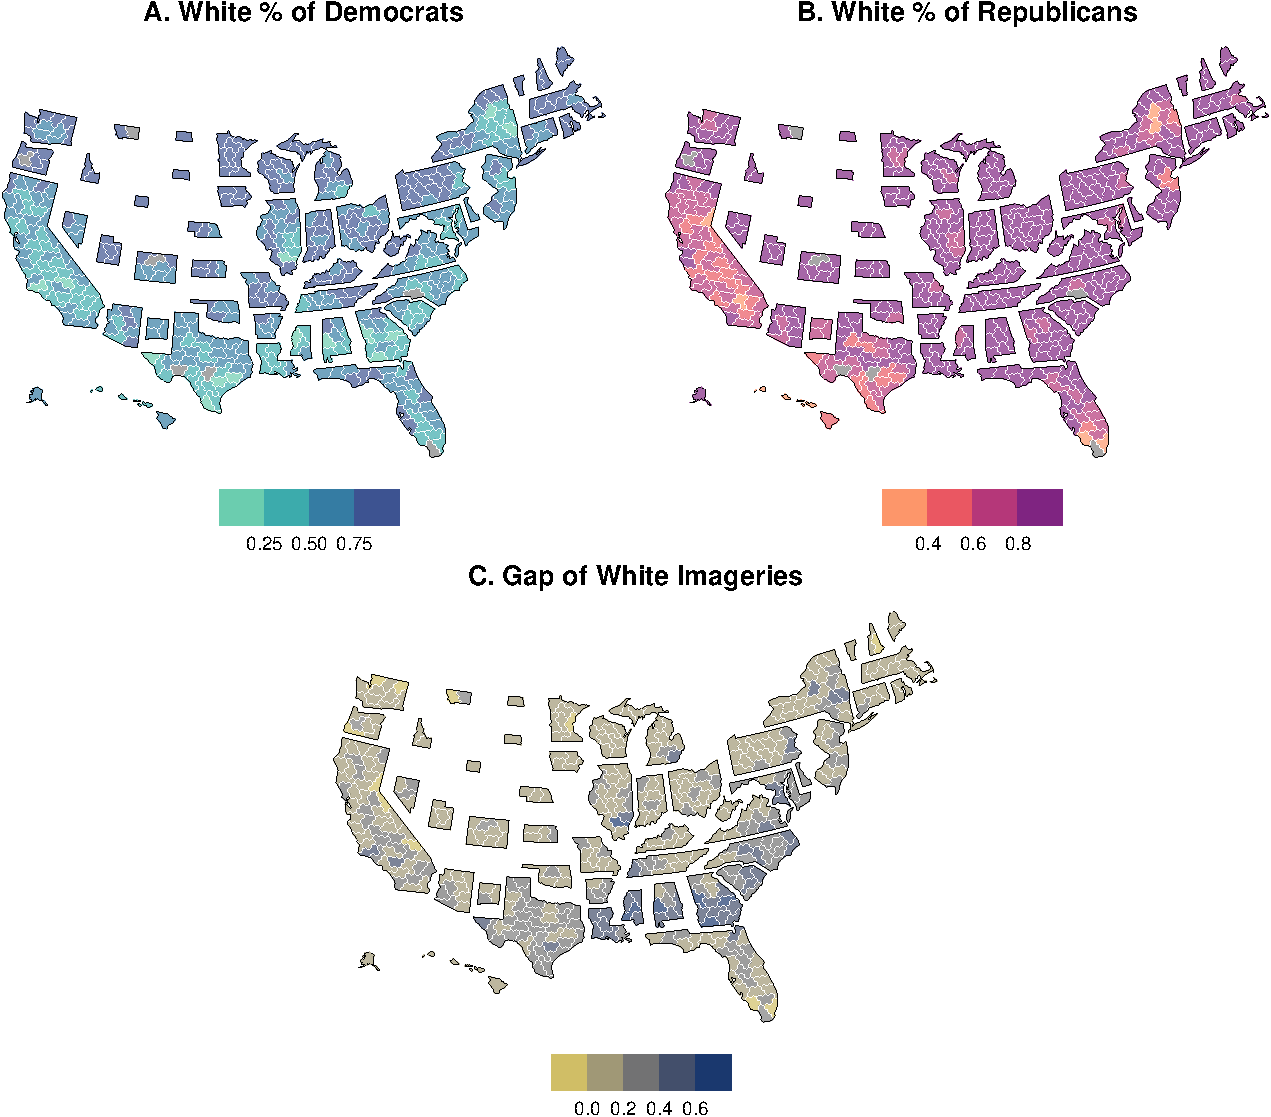
\includegraphics{paper_files/figure-pdf/fig-map-1.pdf}

}

\caption{\label{fig-map}\textbf{Greater contrast of party images
increases the weight of white feelings in voter's affective perception
of the Republican Party.}}

\end{figure}

\begin{figure}[tb]

{\centering 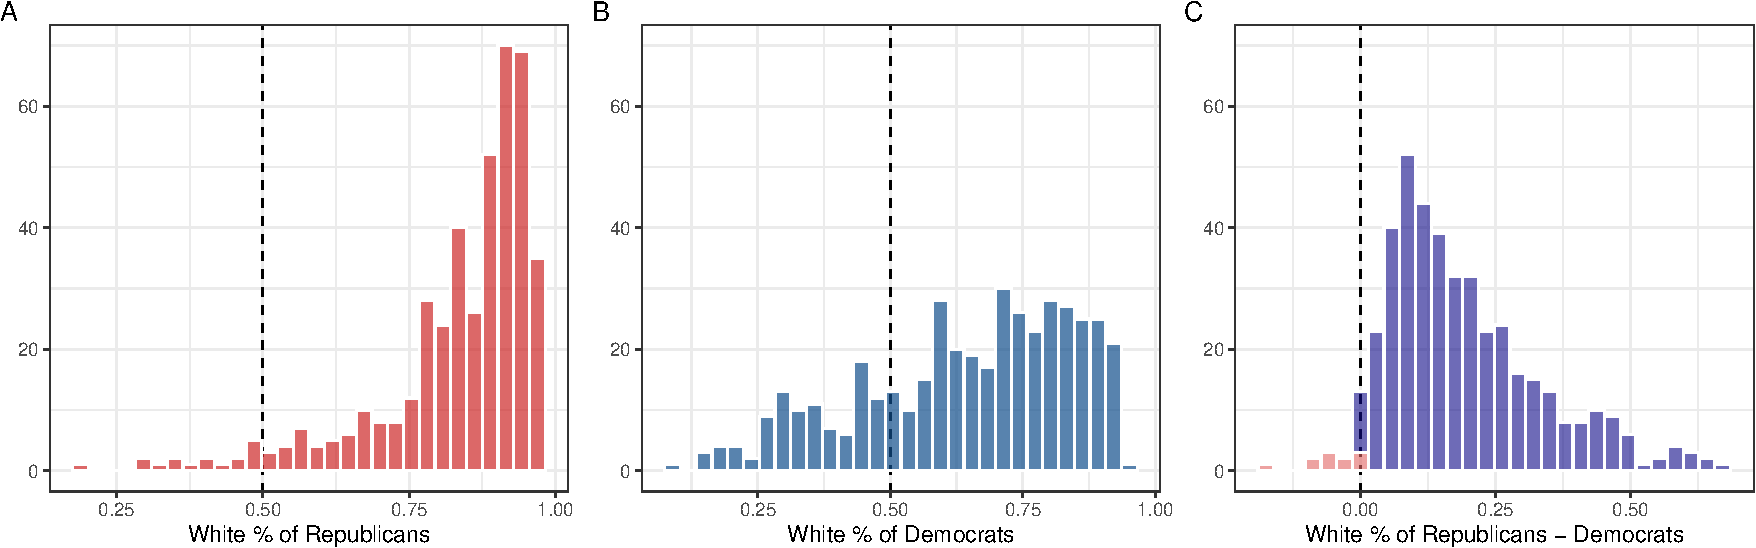
\includegraphics{paper_files/figure-pdf/fig-hist-1.pdf}

}

\caption{\label{fig-hist}\textbf{Greater contrast of party images
increases the weight of white feelings in voter's affective perception
of the Republican Party.}}

\end{figure}

\begin{figure}[tb]

{\centering 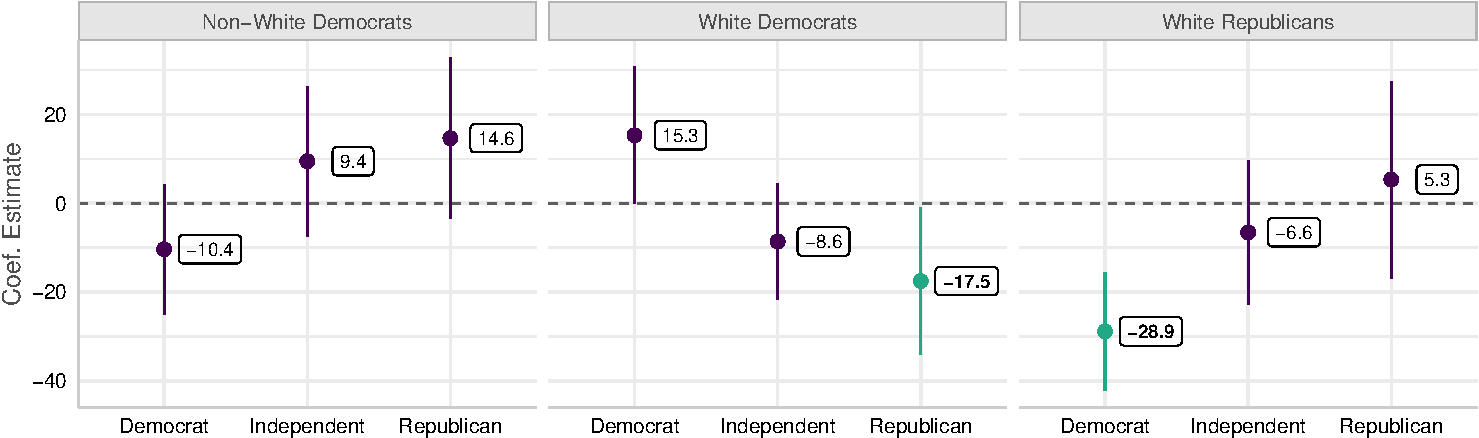
\includegraphics{paper_files/figure-pdf/fig-baseline-1.pdf}

}

\caption{\label{fig-baseline}\textbf{Greater contrast of party images
increases the weight of white feelings in voter's affective perception
of the Republican Party.}}

\end{figure}

\begin{figure}[tb]

{\centering 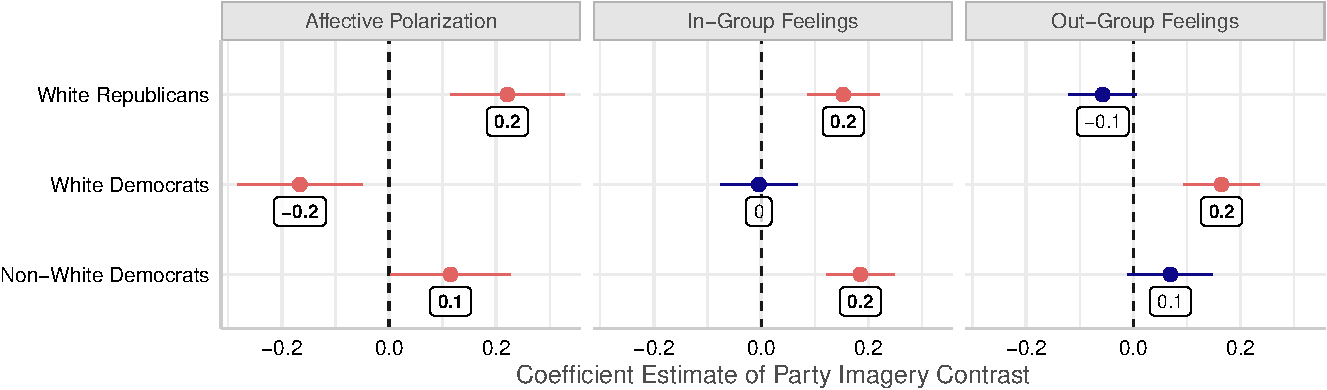
\includegraphics{paper_files/figure-pdf/fig-decompose-1.pdf}

}

\caption{\label{fig-decompose}\textbf{Greater Contrast of Party Images
Increases the Weight of White Feelings in Voter's Affective Perception
of Political Parties}}

\end{figure}

\hypertarget{tbl-mechanism}{}
\begin{table}
\caption{\label{tbl-mechanism}Greater Contrast of Party Images Accentuates the Weight of White
Feelings in Voter's Affective Perception of Politica Parties }\tabularnewline

\centering
\begin{threeparttable}
\begin{tabular}[t]{lccc}
\toprule
  & Republican Feeling & Democrat Feeling & Rep. - Dem. Feeling\\
\midrule
White Feeling Thermometer & 0.188*** & 0.016 & 0.168**\\
 & (0.029) & (0.029) & (0.053)\\
Party Imagery Contrast & 0.019 & 0.195* & -0.183\\
 & (0.089) & (0.089) & (0.162)\\
White Feelings × Party Imagery Contrast & 0.003** & -0.004** & 0.007**\\
 & (0.001) & (0.001) & (0.002)\\
\midrule
Observations & 6983 & 6989 & 6960\\
R squared & 0.053 & 0.033 & 0.046\\
\bottomrule
\end{tabular}
\begin{tablenotes}
\item Note: Robust standard errors in parentheses. + p $<$ 0.1, * p $<$ 0.05, ** p $<$ 0.01, *** p $<$ 0.001
\end{tablenotes}
\end{threeparttable}
\end{table}

\begin{figure}[tb]

{\centering 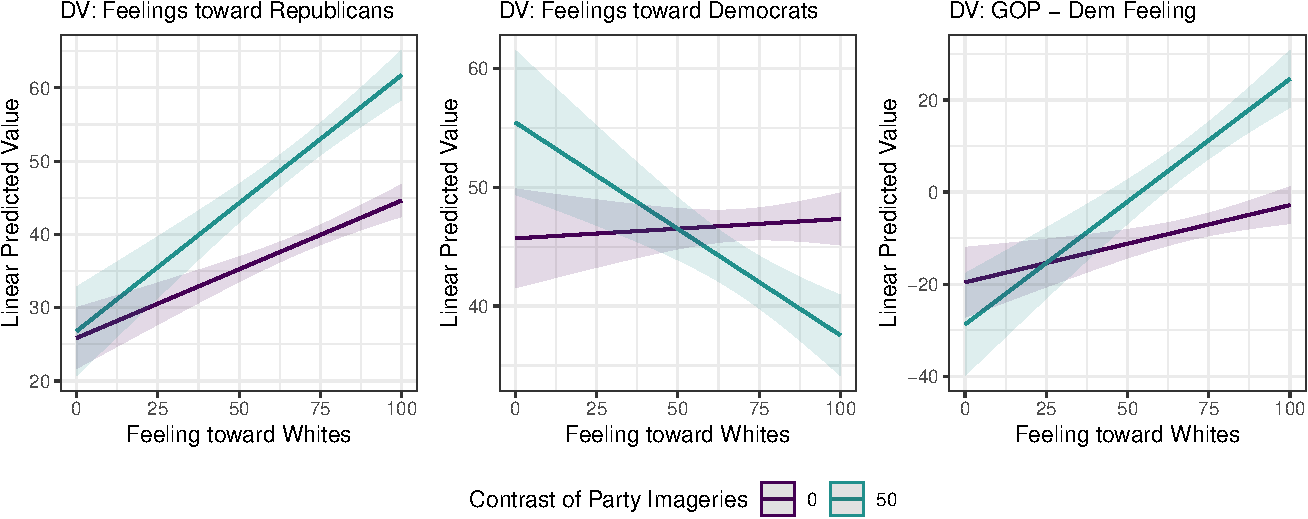
\includegraphics{paper_files/figure-pdf/fig-mechanism-1.pdf}

}

\caption{\label{fig-mechanism}\textbf{Greater contrast of party images
increases the weight of white feelings in voter's affective perception
of the political parties.}}

\end{figure}



\end{document}
